\maketitle
\tableofcontents
\newpage

\section{Zielsetzung}
Ziel des Versuches ist es, den Transport von Wärmeenergie entgegen der Richtung des Wärmeflusses
zu untersuchen. Wichtige dabei zu beachtende Größen sind die Güteziffer, der Massendurchsatz und
die mechanische Leistung des Kompressors.
\section{Theorie}
Die Wärmeenergie in einem abgeschlossenen System fließt von der warmen Umgebung in die kalte
Umgebung. Um diesen Wärmefluss umzudrehen, muss mechanische Arbeit erbracht werden. So
eine Maschine wird als Wärmepumpe bezeichnet. Aus dem ersten Hauptsatz der Thermodynamik kommt
\begin{equation}
    \symup{Q_1 = Q_2 + A}
    \label{eqn:3}
\end{equation}
Das Verhältnis zwischen transportierter Wärmemenge und aufgewendeter Arbeit ist definiert
als Güteziffer $\nu$
\begin{equation}
    % müssen noch überlegen, ob wir die \nu kursiv machen oder nicht
    \nu = \symup{\frac{Q_1}{A}}
    \label{eqn:4}
\end{equation}
Dabei ist A die aufgewendetet Arbeit und $\symup Q_1$ die an das wärmere Reservoir abgegebene
Wärmemenge. Es gilt zu beachten, dass dies die Güteziffer für idealisierte Bedingungen darstellt.
Eine weitere idealisierte Annahme kommt aus dem zweiten Hauptsatz der Thermodynamik
\begin{equation}
    \symup{\frac{Q_1}{T_1} - \frac{Q_2}{T_2}} = 0
    \label{eqn:5}
\end{equation}
Da die Wärmepumpe nicht reversibel arbeiten kann, gilt für die reale Beziehung
\begin{equation}
  \symup{\frac{Q_1}{T_1} - \frac{Q_2}{T_2}} > 0
  \label{eqn:6}
\end{equation}
Nun ergibt sich für \eqref{eqn:4} aus \eqref{eqn:5} und \eqref{eqn:6}
\begin{equation}
  \begin{split}
    % müssen noch überlegen, ob wir die \nu kursiv machen oder nicht
    \nu_{\symup{ideal}} = \symup{\frac{T_1}{T_1 - T_2}} \\
    \nu_{\symup{real}} < \symup{\frac{T_1}{T_1 - T_2}}
    \label{eqn:7}
  \end{split}
\end{equation}
Aus den Messwerten der Temperaturen gegen die Zeit gewinnt man die später genutzte Formel
für die Berechnung der realen Güteziffer
\begin{equation}
    \nu = \frac{\symup dQ_1}{\symup dt N} = (m_1c_w + m_kc_k) \frac{\symup dT_1}{\symup dt \, N}
    \label{eqn:8}
\end{equation}
mit $m_1c_w$ als Wärmekapazität des Wassers in Reservoir 1, $m_kc_k$ als Wärmekapazität
der Kupferschlange und des Behälters und N als gemittelte Leistungsaufnahme des Kompressors.
Die nächste zu betrachtende Größe ist der Massendurchsatz $\frac{\symup dm}{\symup dt}$, der
sich über den Differentialquotienten berechnet
\begin{equation}
      \frac{\symup dm}{\symup dt} = (m_2 c_w + m_k c_k) \frac{\symup dT_2}{\symup dt \, L}
      \label{eqn:9}
\end{equation}
mit L als Verdampfungswärme.
Als letztes kommt die Formel für die mechanische Kompressorleistung $\symup N_{mech}$
\begin{equation}
    \symup{N_{mech}} = \frac{1}{\kappa - 1} \left(p_b\sqrt[\kappa]{\frac{p_a}{p_b}} - p_a \right) \frac{1}{\rho}
    \frac{\symup dm}{\symup dt}
    \label{eqn:10}
\end{equation}
mit $\kappa$ als Verhältnis der Molwärmen und $\rho$ als Dichte des Gases.
\section{Durchführung}
\subsection{Versuchsaufbau}
Der Versuchsaufbau, siehe \ref{fig:1}, besteht aus den beiden thermisch isolierten Reservoiren, deren Temperatur über zwei
digitale Termometer abgegriffen werden. Zwei Rührmotoren sorgen für die gleichmäßige Durchmischung des Wassers.
Der Drücke $\symup P_a$ und $\symup P_b$ lassen sich an zwei Manometern ablesen. Ein Kompressor
mit angeschlossenem Motor stellt die benötigte mechanische Arbeit A bereit; die aufgewendete Leistung zeigt
ein Wattmeter an. Somit lassen sich alle zu messenden Größen erfassen.
\begin{figure}
  \centering
  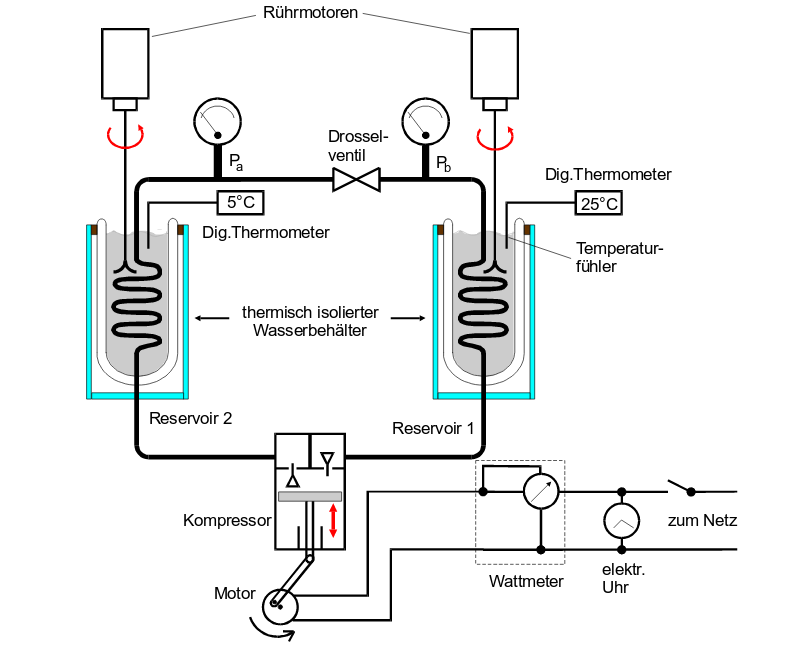
\includegraphics[scale=0.5]{schema.png}
  \caption{Schematische Darstellung des Versuchsaufbaus.}
  \label{fig:1}
\end{figure}
\subsection{Versuchsdurchführung}
Nachdem die Reservoire mit jeweils 3\,$\si{\litre}$ Wasser aufgefüllt wurden,
werden zu Beginn der Messung  die Temperaturen, die Drücke und die Leistung gemessen.
Im $\SI{60}{\second}$ Intervall müssen die oben genannten Größen erfasst werden, bis
$\symup{T_1}$ ungefähr $\SI{50}{\celsius}$ erreicht hat.
\begin{figure}
  \centering
  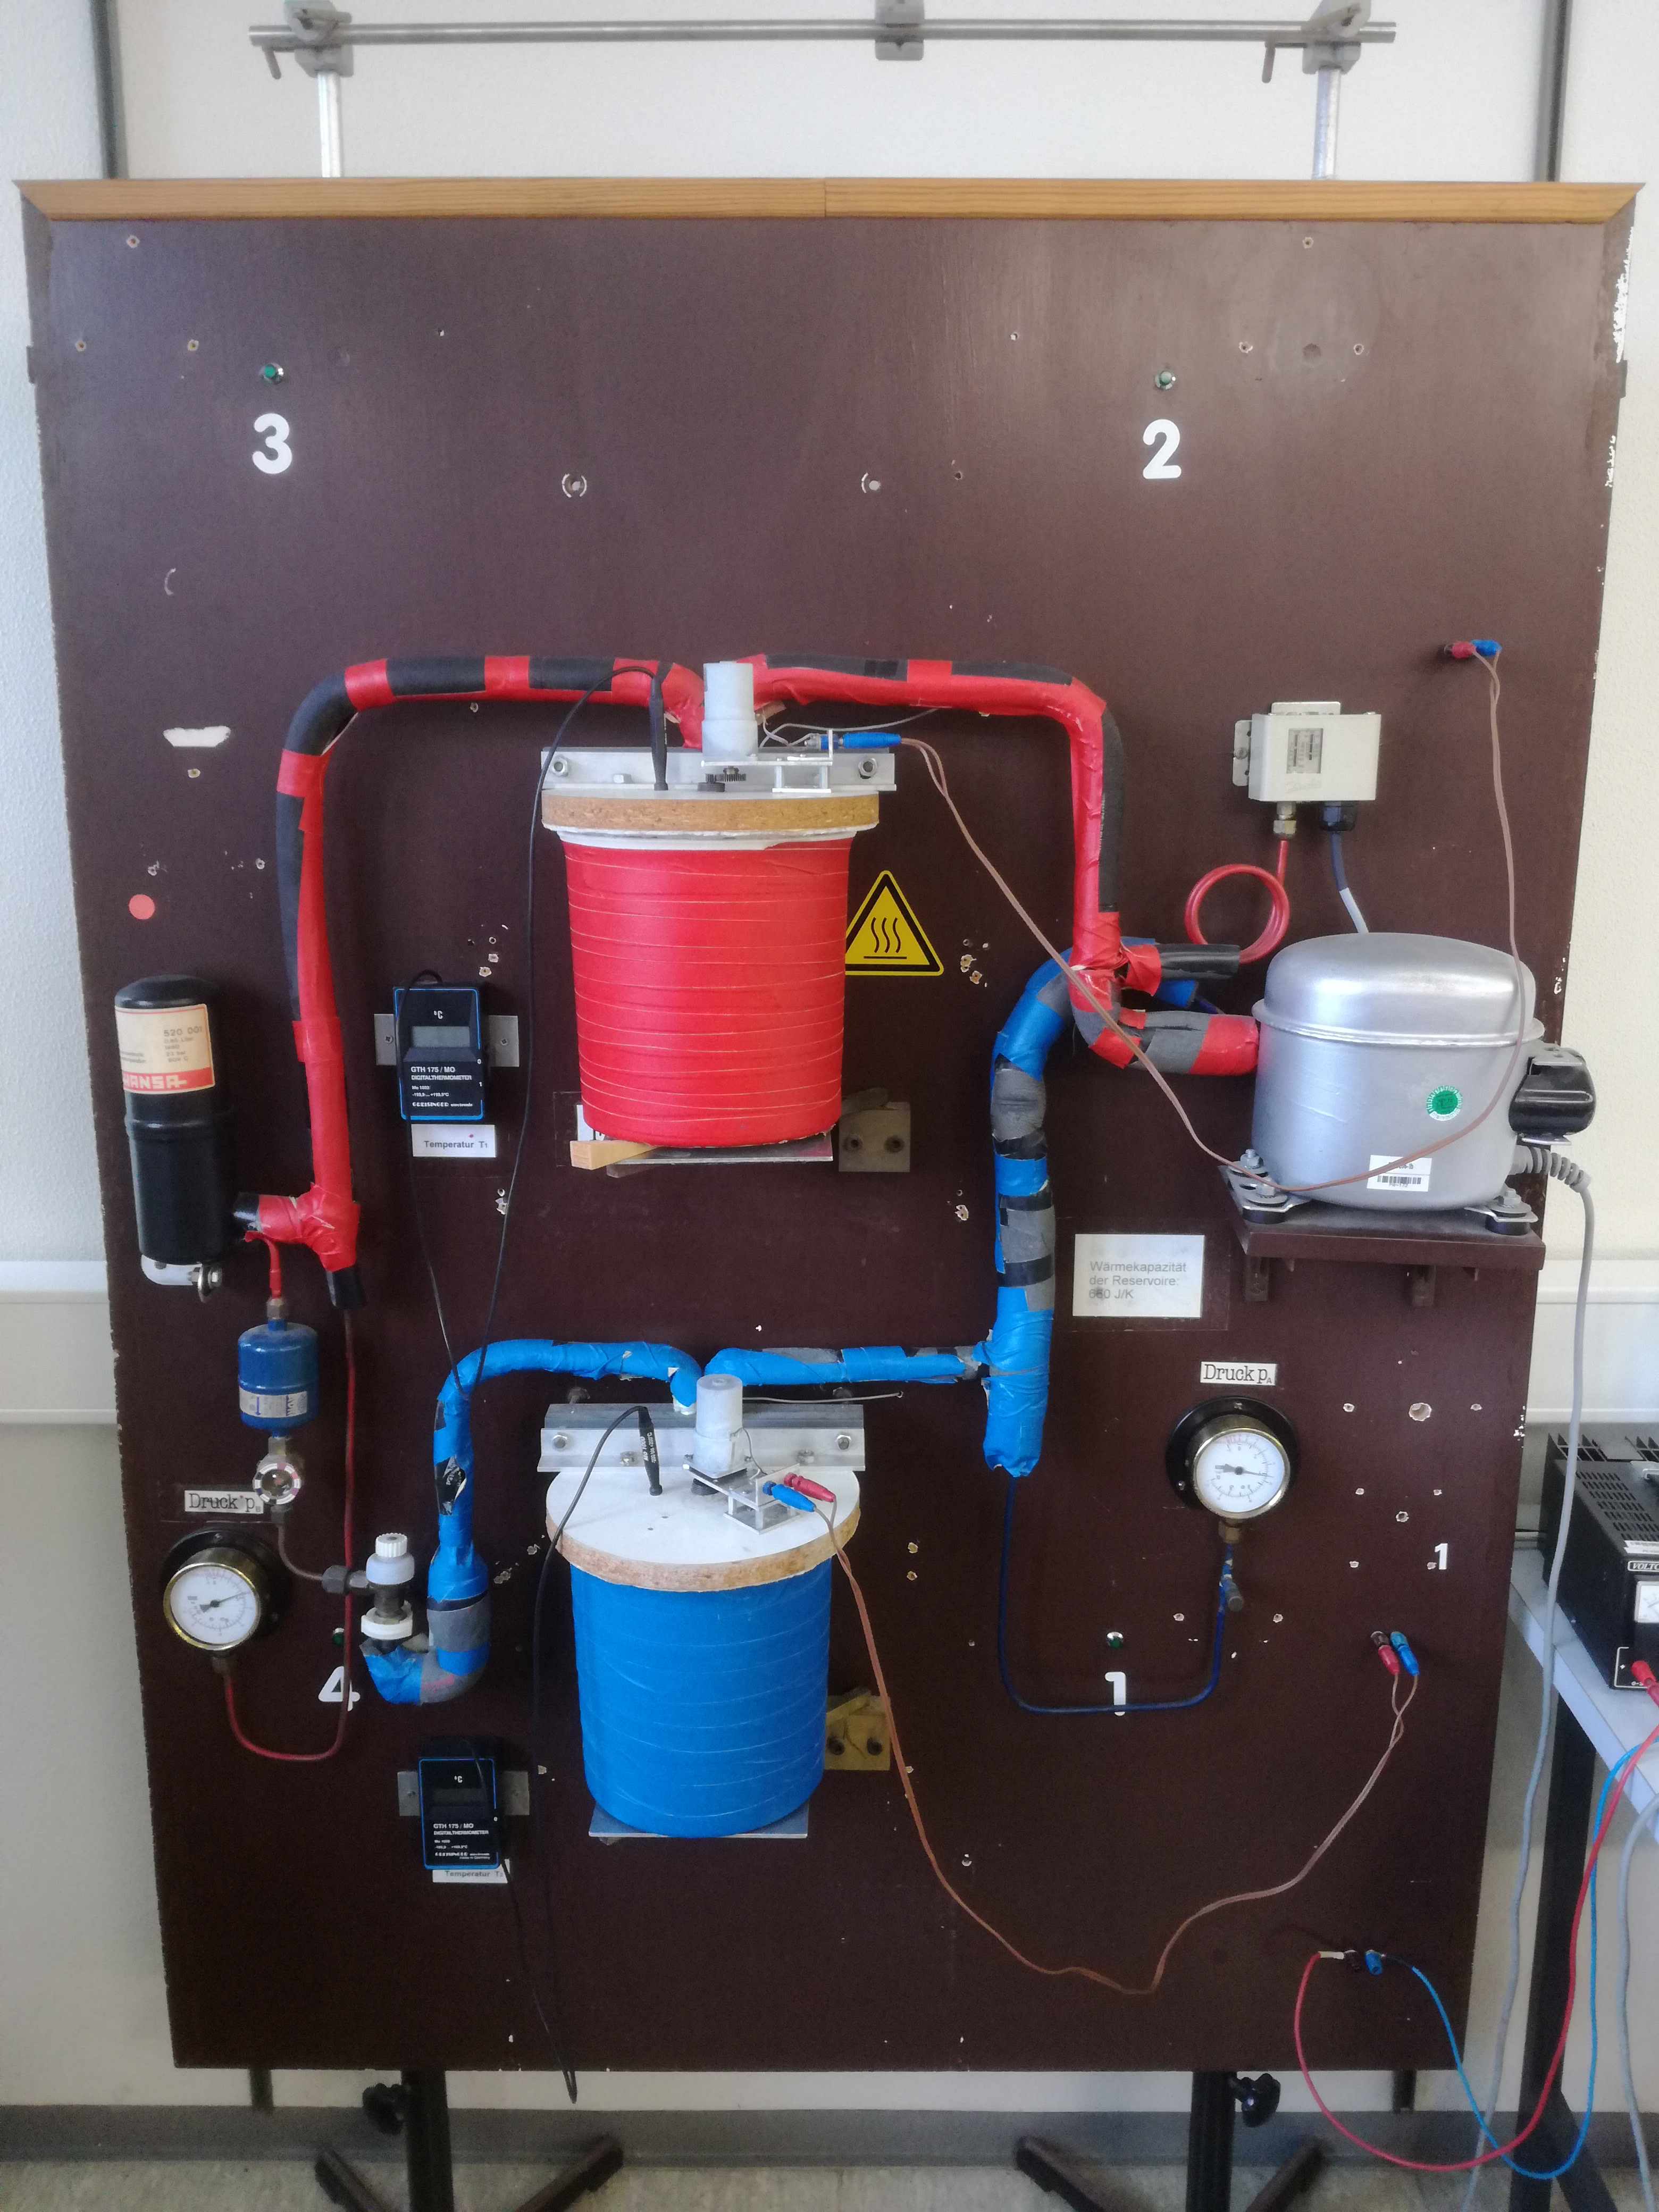
\includegraphics[scale=0.07]{foto.jpg}
  \caption{Der Versuchsaufbau im Foto.}
  \label{fig:2}
\end{figure}
\section{Fehlerrechnung}
Es gibt:
\begin{equation}
  \bar{T} = \frac{1}{n} \sum_{i=1}^{n} T^{i}
  \label{eqn:1}
\end{equation}
den Mittelwert und:
\begin{equation}
  \sigma_{\bar{T}} = \sqrt{\frac{1}{n(n-1)} \sum_{i=1}^{n}(\bar{T}-T_i)^2}
  \label{eqn:2}
\end{equation}
den Fehler des Mittelwertes.

\section{Auswertung}
\label{sec:Auswertung}
\begin{figure}[h]
  \centering
  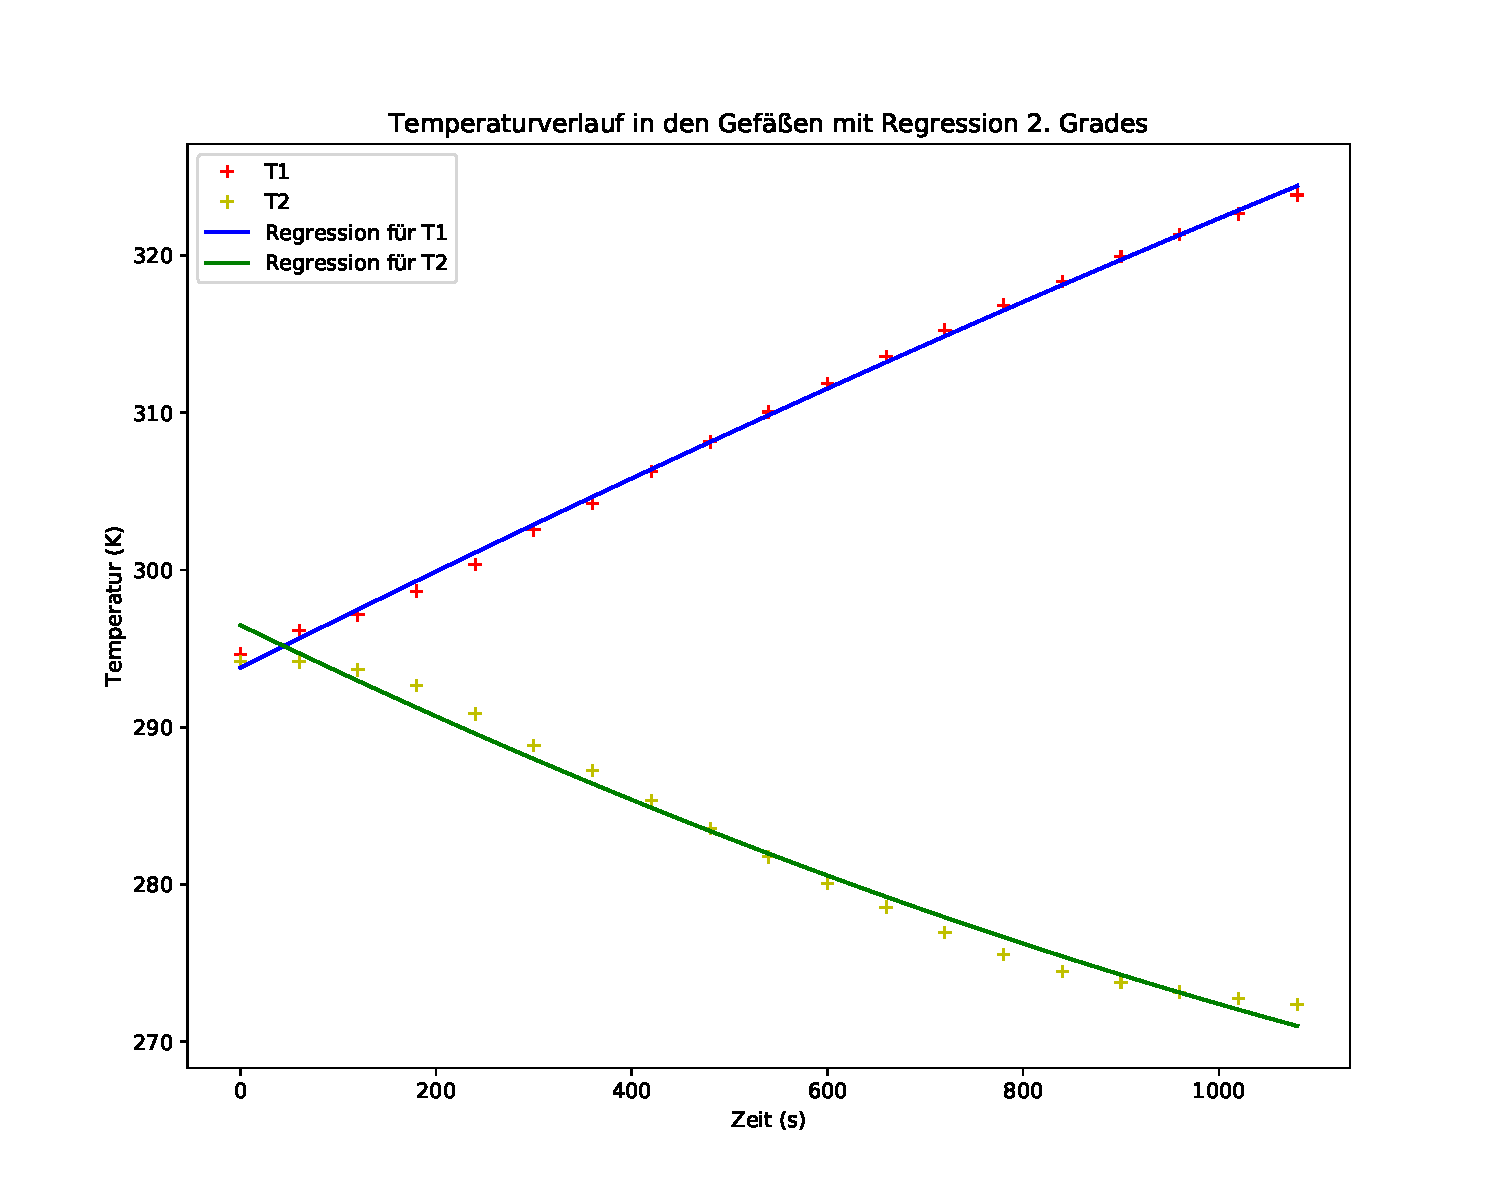
\includegraphics[width=\textwidth]{Grad2.pdf}
  \caption{Temperaturverlauf durch $T(t) = At^2 + Bt + C$ approximiert.}
  \label{fig:3}
\end{figure}
Diese Regression ist, vor allem für die Werte von $T_2$, ungeeignet als Aproximation.
Eine bessere Annäherung erhält man für eine Funktion mit Grad 3, siehe \ref{fig:4}.
Mit diesem Ansatz ist eine vertretbare Approximation gefunden. Die Parameter bestimmen sich nach
\begin{table}
  \centering
  \caption{Parameter für Ansatz $T(t) = At^3 + Bt^2 + Ct + D$, siehe  \ref{fig:4}.}
  \label{tab:1}
  \begin{tabular}{c c c}
    \toprule
    Parameter & $\symup{T_1}$ & $\symup{T_2}$ \\
    \midrule
    A & -1.406E-08 \pm 1.646e-09 & 3.383e-08\pm 2.689e-09 \\
    B & 2.022e-05 \pm 2.707e-06 & -4.869E-05 \pm 4.423e-06 \\
    C & 0.022 \pm 0.001 & -0.007 \pm 0.002 \\
    D & 0.022 \pm 0.001 & 294.704 \pm 0.245 \\
    \bottomrule
  \end{tabular}
\end{table}
\begin{figure}
  \centering
  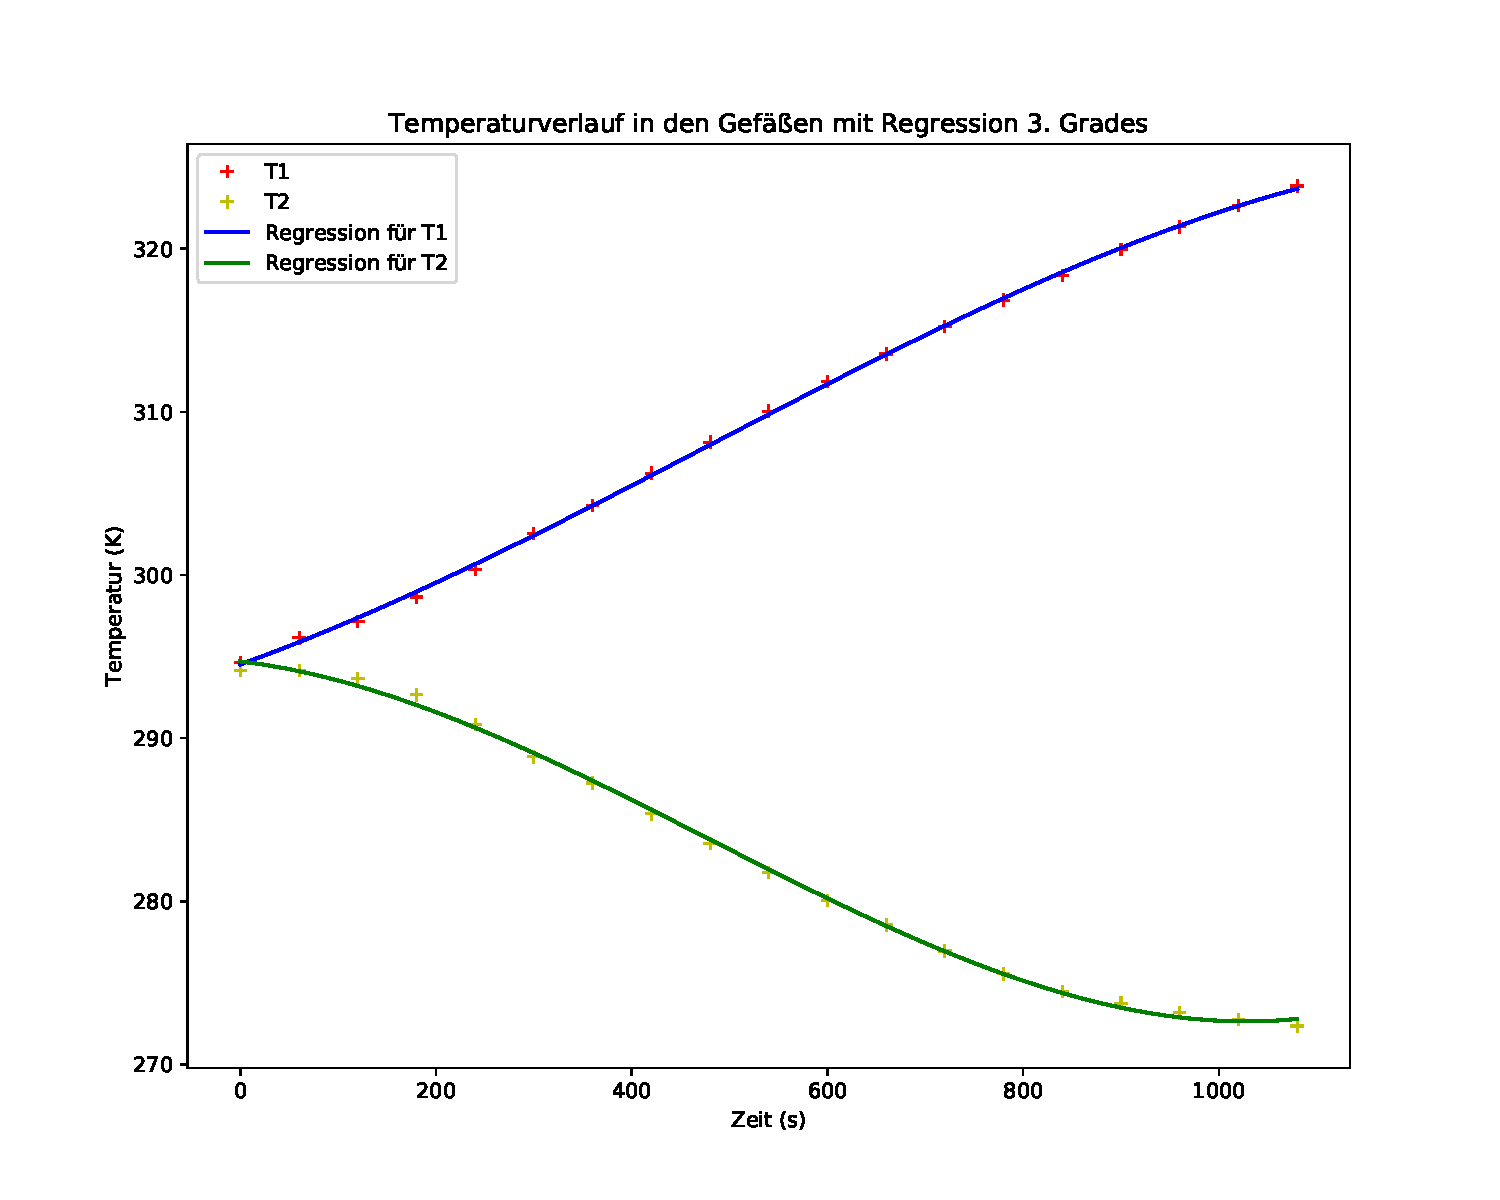
\includegraphics[width=\textwidth]{Grad3.pdf}
  \caption{Temperaturverlauf durch $T(t) = At^3 + Bt^2 + Ct + D$ approximiert.}
  \label{fig:4}
\end{figure}
Für die Differentialqutionten $\frac{\symup dT_1}{\symup dt}$ und $\frac{\symup dT_2}{\symup dt}$
ergibt sich für vier verschiedene Temperaturen:
\begin{table}
  \centering
  \caption{Differentialquotienten $\frac{\symup dT_1}{\symup dt}$ und $\frac{\symup dT_2}{\symup dt}$.}
  \label{tab:2}
  \begin{tabular}{c c c}
    \toprule
    Zeit in $\si{\second}$ & $\frac{\symup dT_1}{\symup dt}$ & $\frac{\symup dT_2}{\symup dt}$ \\
    \midrule
    240 & 0.026 \pm 0.001 & -0.017 \pm 0.002 \\
    480 & 0.028 \pm 0.002 & -0.023 \pm 0.003 \\
    720 & 0.029 \pm 0.003 & -0.025 \pm 0.004 \\
    960 & 0.028 \pm 0.003 & -0.023 \pm 0.005 \\
    \bottomrule
  \end{tabular}
\end{table}

\subsection{Bestimmung der Güteziffer}
\label{Güteziffer}
Für die Güteziffer ergibt sich Formel \eqref{eqn:8} in Vergleich mit der idealen Güteziffer
nach \eqref{eqn:7}
\begin{table}
  \centering
  \caption{Güteziffern der Wärmepumpe für die Zeiten aus \ref{sec:Auswertung}.}
  \label{tab:3}
  \begin{tabular}{c c c}
  \toprule
  Zeit in $\si{\second}$ & $\nu_{\symup{real}}$ & $\nu_{\symup{ideal}}$  \\
  \midrule
  240 & 1.763 \pm 0.097 & 29.998 \pm 2.093 \\
  480 & 1.930 \pm 0.126 & 12.730 \pm 0.882 \\
  720 & 1.985 \pm 0.170 & 8.220 \pm 0.707 \\
  960 & 1.929 \pm 0.224 & 6.622 \pm 0.786 \\
  \bottomrule
  \end{tabular}
\end{table}
Die Wärmekapazität $m_kc_k$ für die Kupferschlange und die Behälter beträgt
$\SI{660}{\joule\per\kelvin}$, die Größe N, also die gemittelte Leistung,
\SI{192.16}{\watt}. Für die spezifische Wärmekapazität $c_w$ ergibt sich nach
\cite{chemie} $\approx \SI{4.19E3}{\joule\per\kilo\gram\per\kelvin}$ mit $m_1 =$
$\SI{3}{\kilo\gram}$.

\subsection{Berechnung des Massendurchsatzes $\frac{\symup dm}{\symup dt}$}
Für den Massendurchsatz ergibt sich nach \eqref{eqn:9}
\begin{table}
  \centering
  \caption{Massendurchsatz $\frac{\symup dm}{\symup dt}$ für die Zeiten aus \ref{sec:Auswertung}.}
  \label{tab:4}
  \begin{tabular}{c c}
    \toprule
    Zeit in $\si{\second}$ & Massendurchsatz $\frac{\symup dm}{\symup dt}$ \\
    \midrule
    240 & -0.0013 \pm 0.0002 \\
    480 & -0.0018 \pm 0.0003 \\
    720 & -0.0019 \pm 0.0003 \\
    960 & -0.0018 \pm 0.0004 \\
    \bottomrule
  \end{tabular}
\end{table}
Die Addition der Wärmekapazitäten ist vom Wert her gleich wie in \ref{Güteziffer},
da $m_2$ auch $\SI{3}{\kilo\gram}$ beträgt und sich ansonsten nichts geändert hat.
Die Bestimmung von L, der Verdampfungswärme, erfolgt indem man den Druck $p_b$
logarithmisch gegen $\frac{1}{T_1}$ aufträgt über lineare Regression die Steigung bestimmt.
\begin{equation}
  \begin{split}
%   ln(p_b) = a \frac{1}{T_1} + b
    m = \SI{-2.45 \pm 0.14}{\kelvin} \\
    b = 10.2 \pm 0.5
   \label{eqn:11}
 \end{split}
\end{equation}
Nach der Formel
\begin{equation}
    L = \frac{-R \cdot m}{M}
    \label{eqn:12}
\end{equation}
ergibt sich für L $\SI{1.68 \pm 0.10E5}{\joule\per\kilo\gram}$.
Dabei ist R die allgemeine Gaskonstante mit dem Wert $R = \SI{8.314}{\joule\per\kelvin\per\mol}$
und $M = \SI{120.9E-3}{\kilo\gram\per\mol}$ die molare Masse des Transportgases.

\subsection{Mechanische Leistung des Kompressors}

\section{Diskussion}
Die Werte für die Temperaturen lassen sich am besten mit einer ganzrationalen
Funktion dritten Grades approximieren, was die verschiedenen Graphen deutlich zeigen.
Diese zeigen, dass die Temperatur zu Beginn und zum Ende der Messung relativ langsam
fallen, dagegen in der Mitte der Messung am schnellsten. Dies passt am besten zu der
oben gennanten ganzrationalen Funktion dritten Grades.
\\
\\
Vor allem die Werte der Güteziffer liegen weit außerhalb des Toleranzbereichs
der Fehlergrenzen. Die realen Güteziffern sind für alle Zeiten kleiner als die
idealen. Dies ist unter anderem darauf zurückzuführen, dass die Reservoire nicht
gut isoliert sind und so ein Wärmeaustausch mit der Umgebung stattfinden kann.
Weiterhin sind die schlecht leitenden Kupferschlangen im Wechselspiel mit einem
ineffizienten Kompressor mögliche Optimierungsmöglichkeiten.
\\
\\
Im Allgemeinen lässt sich sagen, dass die Wärmepumpe wesentlich effizienter arbeiten
könnte als sie es aktuell tut. Als Modell einer Wärmepumpe ist sie jedoch gut geeignet
und anschaulich zu bedienen.
\newpage
\nocite{*}
\printbibliography
